\section{Results and Discussion}

\subsection{Performance Analysis}
If not stated otherwise, benchmarks are written by myself and executed on a intel i5 platform.

\subsubsection{ModernGL}
\vspace{1em}
\begin{minipage}{\linewidth}
    \centering
    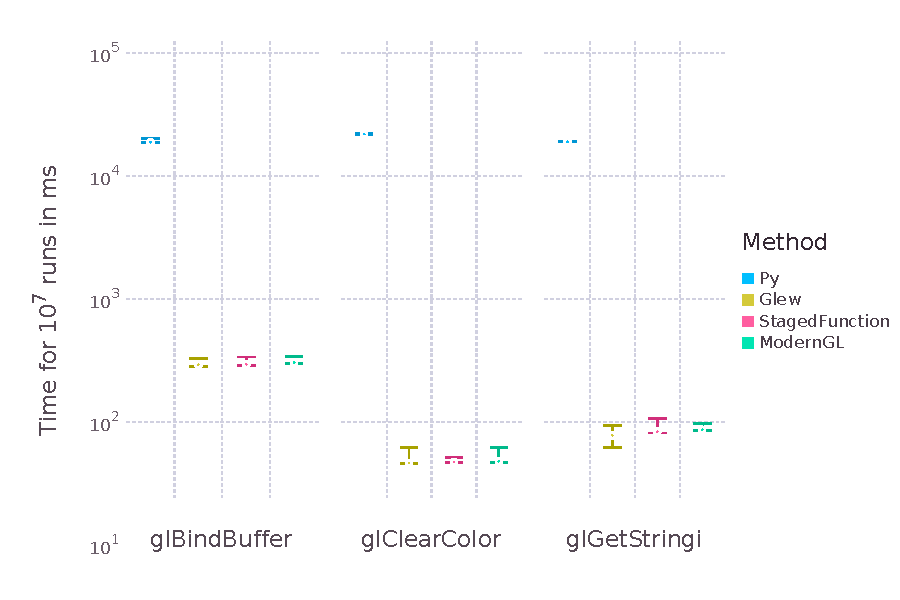
\includegraphics[width=0.9\linewidth]{graphics/glbench.pdf}
    \captionof{figure}[OpenGL Wrapper]{Different performance of OpenGL wrappers. The time for $10^7$ calls was measured 100 times for each function.}
    \label{fig:openglwrapper}
\end{minipage}

\vspace{1em}

\begin{table}[htbp]
    \centering
    \begin{tabular}{l|c|c}
    	\hline
		\textbf{Function} 	& \textbf{Python} 	 & \textbf{Julia StagedFunction} \\
		\hline
		glBindBuffer 		& 64.43  & 1.00 \\
		glClearColor 		& 474.72 & 1.02 \\
		glStringi 			& 244.44  & 1.07 \\
    \end{tabular}
	\captionof{table}[OGL Relative Speed]{Performance relative to C++ with Glew (slowdown, bigger is worse)}
    \label{table:relativespeedoglw}
\end{table}

\subsubsection{Julia}

\vspace{1em}
\begin{minipage}{\linewidth}
    \centering
    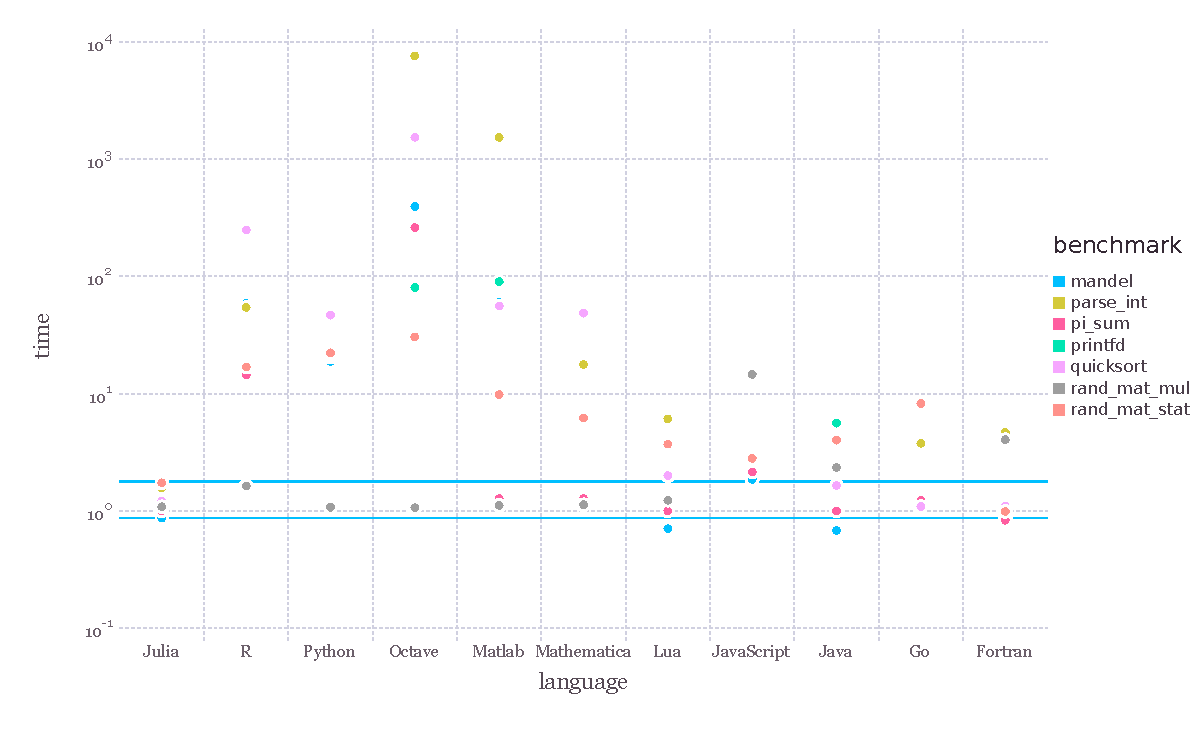
\includegraphics[width=0.9\linewidth]{graphics/juliabench.pdf}
    \captionof{figure}[Julia Performance]{Julia's performance compared to other languages, taken from Julia's micro bench suite \cite{JuliaBench}. Smaller is better, C performance = 1.0.}
    \label{fig:juliabench}
\end{minipage}


\subsection{Extendability Analysis}

The modular design of Romeo has proven to be very effective and the goal of reusability has already proven itself.
Most of the created modules are used independently by different people.
GLVisualize is used by myself for two packages, namely GLPLot, a scientific plotting package for Julia and for a prototype of a file explorer. 
It got forked by several users to create their own dynamic visualization packages.
The same applies for ModernGL and GLAbstraction. Most other used packages are at least used by one other project.
This indicates, that the abstraction and modularity is well designed, so that all the modules can function on their own.

The only exception is GLWindow, which has been used just indirectly through the other packages. 
This can mean three things.
First, it is badly abstracted and doesn't cleanly wrap one use case.
Secondly, it can be, that the use case is not entirely clear to other people, which would not be a big surprise considering the minimal amount of documentation for GLWindow.
And finally, considering the small group of people developing graphics for Julia, it could be that they simply don't need the lower level functionality of GLWindow and instead rely on my other packages that use GLWindow.

This kind of modularity guarantees a broad user and developer base, which in turn results in rich functionality and stability.
From further analyzing the Github repository written or this thesis, one can find out that there is a general lack of documentation.
This hinders people from contributing and using the packages, but could not been 

The implementation in just one language has been achieved by choice. There are only a few exceptions, like the kernel code for OpenGL shaders, which can't currently be written in Julia. 
They can use exactly the same tools and immediately see their results without complicated compilations.
This together with the speed is one of the main achievements compared to other libraries offering similar functionality, like IJulia, VTK and Matlab.
To further proof this point I will analyze the mentioned software in more detail.
For this I will analyze the language usage statistics and necessary tools needed in order to extend the software.
One needs to note, that the statistics of used languages is just a weak indicator for the extendability of a software.
Using different languages for one project can make sense, if the project has different domains, where domain specific languages give an advantage.
This chapter will only discuss the complexity introduced by different languages, which are needed for compatibility with other libraries or because the main language is too slow.

\subsubsection{IJulia}
First of all, IJulia uses ZMQ to bridge the web interface with the Julia instance.
ZMQ is a messaging system using different sockets for communication like inproc, IPC, TCP, TIPC and multicas.
While it is very fast at it's task of sending messages, it can't compete with the native performance of staying inside one language.
This is not very important as long as there doesn't have to be much communication. This changes drastically for animations, where big memory chunks have to be streamed.

using ZMQ(C++), D3, 
Three.js
JavaScript 62.4	 HTML 26.4	 Python 6.9,	 C++ 1.9	 C 1.3,	 GLSL 0.6
D3
JavaScript 95.6	 CSS 4.3
IPython
Python 78.5	 JavaScript 15.1	 HTML 5.0	 Other 1.4

\subsubsection{Paraview and VTK}



This amounts to a total of 3.642.105 lines of code written in 29 languages.

\subsubsection{Matlab}



\subsection{Usability Analysis}
